
% to choose your degree
% please un-comment just one of the following
\documentclass[bsc,frontabs,twoside,singlespacing,parskip,deptreport]{infthesis}     % for BSc, BEng etc.
% \documentclass[minf,frontabs,twoside,singlespacing,parskip,deptreport]{infthesis}  % for MInf

\usepackage{graphicx}
\usepackage{float}
\usepackage{url}

\begin{document}

\title{Sensing Spaces: Personal Exposure to Air Pollution with Different Modes of Transport and Urban Environments Using Wearable Sensors}

\author{Mihai Visuian}

% to choose your course
% please un-comment just one of the following
%\course{Artificial Intelligence and Computer Science}
%\course{Artificial Intelligence and Software Engineering}
%\course{Artificial Intelligence and Mathematics}
%\course{Artificial Intelligence and Psychology }   
%\course{Artificial Intelligence with Psychology }   
%\course{Linguistics and Artificial Intelligence}    
\course{Computer Science}
%\course{Software Engineering}
%\course{Computer Science and Electronics}    
%\course{Electronics and Software Engineering}    
%\course{Computer Science and Management Science}    
%\course{Computer Science and Mathematics}
%\course{Computer Science and Physics}  
%\course{Computer Science and Statistics}    

% to choose your report type
% please un-comment just one of the following
%\project{Undergraduate Dissertation} % CS&E, E&SE, AI&L
%\project{Undergraduate Thesis} % AI%Psy
\project{4th Year Project Report}

\date{\today}

\abstract{
This is an example of {\tt infthesis} style.
The file {\tt skeleton.tex} generates this document and can be 
used to get a ``skeleton'' for your thesis.
The abstract should summarise your report and fit in the space on the 
first page.
%
You may, of course, use any other software to write your report,
as long as you follow the same style. That means: producing a title
page as given here, and including a table of contents and bibliography.
}

\maketitle

\section*{Acknowledgements}

I would like to thank my supervisor, professor D K Arvind for his main support in helping me work thoroughly on a project of such high complexity and importance in the real world. I would also like to thank him for his valuable advice and guidance.

Furthermore, I would like to thank Andrew Bates for his support in providing equipment and helping with maintenance of sensors and servers.

More acknowledgements to follow.....

\tableofcontents

%\pagenumbering{arabic}


\chapter{Introduction}

\section{Motivation}

Air pollution in large urban environments is a controversial topic nowadays and pollution sources, as well as distribution and effect on human health have been widely studied. Particulate matter (PM) represents the sum of all solid particles and liquid droplets of small sizes that are suspended in the air. It has been discovered that exposure to such particles of size less than 10 microns can be hazardous for the human body and it has been associated with increased mortality rates in areas labelled as highly polluted \cite{Dockery1994}.

Air quality is mostly measured through stationary Air Quality Monitoring Stations (AQMS). They measure air quality at a fixed location on a certain radius with high precision. Data collected from such networks of stations distributed strategically within urban environments is used to determine exposure to pollutants and is used for checking if a specific area meets requirements set by legislation. One drawback of this approach is that monitoring a large fixed region through a stationary sensor would not always suffice to obtain accurate information about air quality and pollution sources, as parameters vary from a corner of the region to another and other external factors such as wind speed and terrain type affect the results.

One approach to solve this issue and obtain more accurate data from the environment would be to deploy low-cost mobile sensors on people, such as drivers, pedestrians and cyclists in order to obtain a more precise spatial representation of the air quality. However, these sensors have to be calibrated in correlation with the Air Quality Monitoring Stations to ensure high precision of the information gathered.

\section{Objectives}

This project mainly focuses on Mobile Exposure Monitors (MEM) developed by the Centre for Speckled Computing. These wearable devices are equipped with sensors measuring humidity, temperature and particulate matter. Data is transmitted to an Android device via Bluetooth Low Energy. The project presents several study methods for detecting urban environments and personal exposure with different means of transport, based on air quality data collected with the wearable sensors. The objectives of the project are:

\begin{itemize}
\item Collect data at specific times on a daily basis and on a fixed route.
\item Perform analysis on data gathered for various modes of transport and urban environments and research machine learning techniques to detect personal exposure on a specific mode of transport or urban environment based on temperature, humidity and particulate matter attributes.
\item Build a data visualization tool for a more accurate spatial representation of data gathered and results obtained after applying statistical and machine learning methods.
\item Validate measurements of sensors against a more accurate Air Quality Monitoring Station in Edinburgh.
\end{itemize}

\section{Literature Review}

There are past studies concerning exposure of cyclists to air pollution and traffic noise in central neighbourhoods of Montreal \cite{Apparicio201663}. Despite it is known that cycling in urban areas would have beneficial effects on people's health, it is associated with potential health risks due to long time exposure to polluted air and traffic noise. The focus of this study was to analyse exposure of cyclists to air pollution and traffic noise and detect the impact on exposure of local factors such as weather conditions and the type of roads. A number of 85 bicycle trips were analysed, totalling 422 km of travel. The results revealed a weak negative correlation between noise and air pollution (NO$_2$) measures of exposure.

A study \cite{Dirks2012} done in Auckland, New Zealand, examined personal exposure to air pollution, namely carbon monoxide (CO) for several modes of transport, using Langan T15n \cite{Langan} portable carbon monoxide monitors. Participants were constrained to travel at specific peak traffic times between designated start and end points. Results suggest that lowest exposure to CO particles are experienced by train commuters, while motorcyclists were exposed to significantly higher average concentrations. Furthermore, travel by bus on a dedicated route proved to be more effective than travel by car on a congested motorway. Also, average exposure of cyclists and pedestrians proved to be similar to bus and car commuters. However, when increased physical activity that implies higher volumes of air breathed, along with increased commuting time were taken into account, air pollution dosage became much higher than for the motorised means of transport.

Most research regarding particulate matter has been performed in terms of values of PM2.5 and PM10, namely measurements of mass particulates with lower dimensions than 2.5 and 10 microns. A study \cite{Cho2008} is concerned about the relationship between mortality rate and particulate matter measured in Seoul, South Korea by an Optical Particulate Counter (OPC) and a national monitoring station. Particulate matter (PM2.5 and PM10) and particle counts from 0.3 to 25 microns were measured. The results concerning particle counts were associated with a 5.73\% and 5.82\% in mortality caused by respiratory diseases.

\section{Method}

Data collection has been performed in several phases, using a monitoring device worn around the chest, measuring particulate matter (PM1, PM2.5 and PM10 values along with particle counts of different sizes), as well as temperature and humidity. The sensor communicates with an Android device via Bluetooth to which the data gathered is sent. First, data was gathered on Nicholson Street while using a taxi to Calton Hill during midday. Then, data was gathered while walking on the same route, at the same time of the day, in order to perform the first classification analysis between different means of transport (walking as opposed to cars). For further investigation of personal exposure with different modes of transport, another set of data collected was obtained from a train trip from Edinburgh to London King's Cross, including a bus trip to Edinburgh Waverley, as well as walking trips in Edinburgh, London and London Underground.

Data analysis has been performed using Python and Jupyter Notebooks. First, the raw data was labelled accordingly in terms of the mean of transport used at each point in time. Secondly, the raw data was checked for any outliers existing in all the values of interest. After removing all irrelevant outliers, several machine learning classifiers have been used on PM data, along with temperature and humidity, in order to perform a classification of means of transport used during personal exposure experiments.

As far as personal exposure with different urban environments is concerned, a data collection schedule has been organised on a route in Edinburgh, including Nicholson Street, Melville Drive, Middle Meadow Walk, Tollcross and Lauriston Place, so that all types of urban environments would be detected. More exactly, the same route was covered over a week at two different times of the day, first at midday, during lunchtime between 13:00 and 14:00 and then in the evening, between 17:00 and 18:00, when a traffic peak hour is most probable to occur.

As in the previous set of experiments, Jupyter Notebooks have been used for analysis of the dataset regarding different urban environments. In this case, unsupervised machine learning methods have been applied for classification of data, as ranges of PM values corresponding to each urban environment type vary from a region to another. Thus, K-means clustering was performed first on the coordinates of the dataset features, such that all samples would be grouped into compact clusters and the mean values of the PM related values would be computed for each cluster. Then, a second K-means clustering was applied to the mean values of the clusters obtained in the previous step in order to detect the different types of urban environments.

\section{Structure of the Report}

Chapter 2 reveals detailed information regarding equipments used in the data collection phase, as well as details about PM measurements obtained. Moreover, details about the modes of transport used and types of urban environments taken into consideration are presented.

Chapter 3 details the data collection phase. Then, it also introduces details about statistics and machine learning techniques used in the data analysis process. Moreover, it introduces a data visualization tool implemented from scratch to ease analysis of data collected. Details about this tool will be further discussed in the following chapter.

Chapter 4 details on the data visualization tool, focusing both on the purpose and the functionality of the tool. The application is formed of two main parts, namely the front-end dealing with the spatial representation of the data on a map and the back-end, which consists of an API creating requests to the data collected which is stored in a database.

Chapter 5 presents the results obtained from the data analysis phase. First, a research regarding classification of pollution exposure with different modes of transport is done using various machine learning classifiers. Then, unsupervised data is used to detect several types of urban environments, which will be presented in detail in chapter 2.

Finally, chapter 6 presents the conclusions drawn from the results obtained from data analysis and described in detail in chapter 5. Moreover, potential improvements and further study areas regarding the main topic of the project worth exploring are described.

\chapter{State of the Art}

\section{Mobile Exposure Monitor}

The Mobile Exposure Monitor (MEM), called AirSpeck-P is a wearable device developed with the purpose of quality of environment measurement by the Centre for Speckled Computing. It is equipped with sensors measuring particulate matter counts and mass (Alphasense OPC-N2), as well as temperature and humidity (Sensirion SHT-75). The device transmits sensor readings via Bluetooth Low Energy (BLE) technology to a smart phone or tablet \cite{airspeck}. The latest firmware of the device is also equipped with a light sensor, measuring light intensity. The MEM is adapted to a running belt, so that it could be easily worn during data collection. Figure \ref{fig:airspeck} presents the AirSpeck device attached to the running belt, along with the placement of each sensor.

\begin{figure}[h!]
  \center
  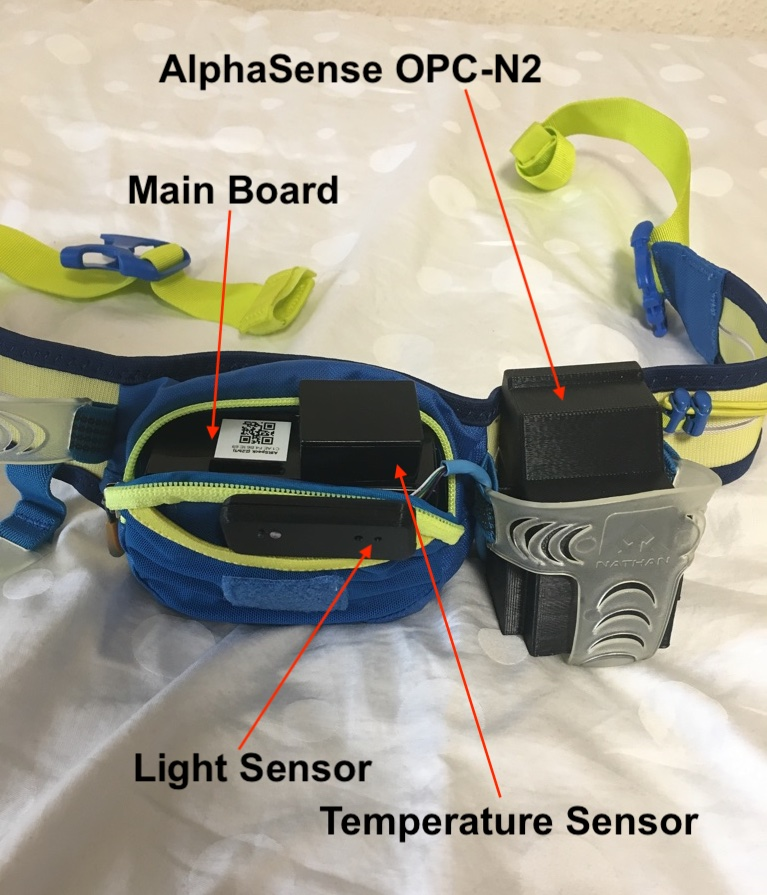
\includegraphics[width=\columnwidth]{airspeck.jpeg} 
  \caption{This picture presents the AirSpeck mobile exposure monitor along with the layout of all the sensors attached to a running belt.}
  \label{fig:airspeck}
\end{figure}


\subsection*{Alphasense Optical Particle Counter}

The data gathered via the Alphasense OPC-N2 \cite{opc} represents the main subject of interest in this project. Size-resolved particulate matter counts are measured in real time, with the latest version of the sensor sampling the environment every 10 seconds. The sensor detects particulates in the range from 0.38 to 17 microns and separates them in 16 different ranges depending on their size \cite{airspeck}. Each range is referred to as a bin, and every bin has a particulate count measurement for the given sampling period. The OPC uses a laser beam and measures the light scattered by individual particulates to determine particulate sizes and counts. PM1, PM2.5, and PM10 measured in $ \mu g /m^3 $ are calculated from the number concentrations detected, assuming negligible contribution from particulates of size less than the lower limit of 0.38 microns.


\subsection*{Temperature Sensor}

A Sensirion SHT-75 temperature and humidity sensor \cite{sensirion} is included on the AirSpeck printed circuit board (PCB) to enable temperature and humidity monitoring without the need to connect to external sensors. The sensor is contained in a waterproof (sintered metal) enclosure \cite{airspeck} and it is placed to protrude outside the enclosure, so that an accurate reading of the temperature and humidity values in the ambient air is ensured.


\subsection*{Communication}

The AirSpeck device has a built-in Bluetooth Low Energy (BLE) radio which communicates with a custom Android application on the mobile device, utilised for receiving and labelling the the sensor readings with time and location (GPS) information. The sensor readings are saved locally in CSV files and they are also forwarded to a remote server for analysis either via cellular network or WiFi.

\section{Urban Environments}

As far as urban environments detection is concerned, five different types of urban environments are taken into consideration in terms of the average values of the sensor readings regarding particulate matter:

\begin{itemize}
\item Park Paths - they are referred to green areas and paths within parks. One example that was constantly scanned with the purpose of studying personal exposure to different urban environments is the North Meadow Walk in the Meadows Park in Edinburgh, also highlighted in Figure \ref{fig:december_route}.

\item Pedestrian Areas - they are referred to roads accessible only to pedestrians such as the Middle Meadow Walk portion between Lauriston Place and George Square Lane, also highlighted in Figure \ref{fig:december_route}.

\item Quiet Roads - they represent quiet roads in the city with little or non-existent traffic.

\item medium traffic areas - they represent streets with medium traffic during the day, such as Melville Drive.

\item crowded / high traffic areas - they represent crowded areas with intense traffic during the day. They are located especially in the city centre and they mostly exist around junctions such as Tollcross or the cross-roads between Princes Street and Telford Road in the West End. 
\end{itemize}
\label{list:urban-environments}

\section{Personal Exposure with Modes of Transport}

In order to study personal exposure in all cases, six different exposure situations corresponding to six different modes of transport used have been taken into consideration during the data collection process:

\begin{itemize}

\item Pedestrian Data - this represents sensor readings gathered from subjects wearing the AirSpeck device while walking around key areas in Edinburgh, described more thoroughly in \ref{sec:data-collection}.

\item Car - air quality data was collected by Mark Miller (a member of the Centre for Speckled Computing) with the AirSpeck while commuting to work by car in Edinburgh. More details about the routes are presented in \ref{sec:data-collection}.

\item Train - data was also gathered while travelling by train on different routes (From Edinburgh to London and Manchester respectively).

\item Bicycle - bicycle data is composed of two different datasets. One represents data that was collected during the summer of 2015 by Aart Meijer, an MSc student while commuting to university by bicycle. Another dataset was gathered in February, during the snow storm. More details regarding the paths are emphasised in \ref{sec:data-collection}.

\item Bus - data was also collected while travelling by bus on different routes around Edinburgh which will be further detailed in \ref{sec:data-collection}. One of the bus routes on which scanning was performed is shown in Figure \ref{fig:bus_route}.

\item subway (in London) - a small amount of sensor readings were gathered while travelling by subway in London. However, the ambient air scanning was performed during only one trip and hence, this dataset contains few inputs.
\end{itemize}

\chapter{Methodology}

\section{Data Collection Process}
\label{sec:data-collection}

To begin with, the Mobile Exposure Monitor transmits sensor readings to the Android device through the Airspeck app, via Bluetooth Low Energy. Values obtained from OPC measurements are sent every 10 seconds along with GPS coordinates. This ensures an effective spatial representation of the created datasets especially when data is collected at walking speed.

\subsection{Training Dataset Creation}
\label{subsec:training-dataset}

During the project development, an annotated dataset with modes of transport used at each point was created for data analysis. Each data point contains information about the temperature, humidity, GPS coordinates and accuracy, along with PM1, PM2.5, PM10 values and particulate matter counts split into 16 bins. Most of the data was collected in the first semester, more exactly during November and December. First data collection was performed during a train journey from Edinburgh to Manchester, on a route between several train stations for one hour.

Moreover, a major phase of data collection involving the analysis of different types of urban environments occurred between the 3rd and the 8th of December. More precisely, data capturing particulate matter counts had been collected using the MEM, by walking on a fixed route around meadows based on a daily schedule for a week (Figure \ref{fig:december_route}). The route was scanned twice a day, both during lunch time between 13:00 and 14:00 and in the afternoon between 17:30 and 18:30, so that the same path would be examined at different times of the day involving different intensities of the traffic.

\begin{figure}[h]
  \center
  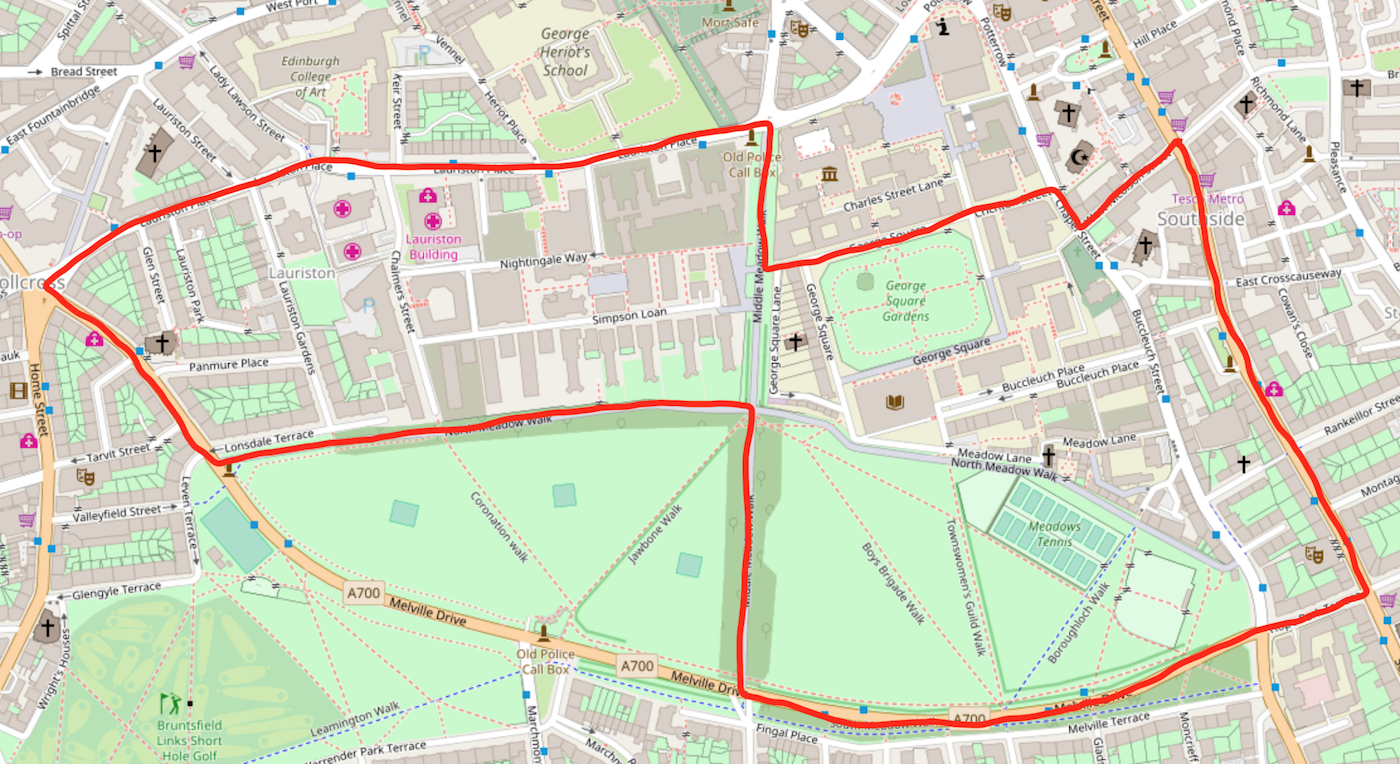
\includegraphics[width=\columnwidth]{december_route.png} 
  \caption{This map of Meadows region emphasises the route that was scanned while walking in December based on the schedule mentioned.}
  \label{fig:december_route}
\end{figure}

More data gathered and annotated with the purpose of studying personal exposure with different modes of transport has been obtained from Mark Miller who commuted to work by car and wore the device for two consecutive days. He also used the sensors on a train journey to London and around the city centre, involving bus and subway transport. Hence, such a data addition helped balance the categories in the final dataset representing the modes of transport used.

Moreover, more data was collected by bus several times. Firstly, a similar route as the one scanned by Mark Miller (Figure \ref{fig:bus_route}) was taken into account in order to test the types of environment encountered on the route and to balance the final training dataset with the addition of new bus tagged data points. Then, a second bus route between St Andrews Square and Queensferry was taken into account for scanning. The latter data collection session involved the gathering of both pedestrian and bus labelled inputs and a part of these data points were included in the validation sets described in \ref{subsec:test-data-collection}.

\begin{figure}[h!]
  \center
  \includegraphics[width=\columnwidth]{bus_route.png} 
  \caption{This map emphasises the route that was scanned while taking the bus several times from Waverley station towards Princes Street, George Street and Telford Road.}
  \label{fig:bus_route}
\end{figure}

Furthermore, Aart Meijer, an MSc student whose honours project involved air quality prediction using wearable sensors on cyclists collected data on a fixed route around Meadows when he was commuting to university every day by bicycle. A part of the dataset containing approximately 1000 data points has been extracted and compared in \ref{subsec:different-weather} to a new set of data points collected in the evening of the 26th of February 2018 (Figure \ref{fig:february-bike}), during the beginning of the snow storm, in order to analyse how different weather conditions affect sensor readings of particulate matter related information.

\begin{figure}[h!]
  \center
  \includegraphics[width=\columnwidth]{bike_feb.png} 
  \caption{This map emphasises the route that was scanned while taking the bicycle on the 26th of February, during the beginning of the snow storm.}
  \label{fig:february-bike}
\end{figure}

\subsection{Test Data Collection}
\label{subsec:test-data-collection}

Apart from data gathered from different urban environments and by using different modes of transport with the aim of creating a balanced and annotated training dataset used in supervised learning methods for classification of means of transport, more data has been collected and labelled by other users of the AirSpeck device with the purpose of further validating the classification methods created. The classification results for the validation dataset are thoroughly described in \ref{subsec:results-urban-env-use}.

As previously mentioned in \ref{subsec:training-dataset}, a part of the data points gathered along the bus route between St Andrews Square and Queensferry was used only for validation, along with pedestrian tagged inputs that were collected during the trip between bus stations on Princes Street and in Queensferry. Moreover, the trip also included a 12 minute bus journey from Nicholson Street to Princes Street, which was entirely used for validation.

Moreover, walking data was collected on the 28th of February by different subjects during the night around the Meadows Park. All the inputs gathered in this session were used for validation.

Furthermore, new inputs were collected for validation on a train journey to London for about three hours on the 15th of March. A percentage of 25\% of the data points were included in the training dataset with the purpose of balancing the distribution of the labelled inputs by adding more train tagged points. The rest of the data gathered was used entirely for validation.


\section{Data Analysis}
\label{sec:data-analysis}

\subsection{Raw Data Information}

The entire training dataset contains initially a total of 6423 data points. However, there exist points that have missing information related to important attributes such as null temperature and humidity values or null particulate matter counts over the entire series of 16 bins. Thus, these outliers have been removed before proceeding to any experiments as described in \ref{subsec:outlier-removal} and hence, the final, sanitized dataset contains 5409 data points. Figure \ref{fig:distribution} shows the distribution of the training dataset in terms of the labels representing the modes of transport used. As it could be observed, the data points distribution over the \textit{on foot}, \textit{train}, \textit{bike} and \textit{bus} labels is balanced as the training dataset contains roughly over 1100 inputs of each type.

\begin{figure}[h!]
  \center
  \includegraphics[width=0.6\columnwidth]{distribution.pdf}
  \caption{This histogram presents the distribution of the data points in terms of the modes of transport labels.}
  \label{fig:distribution}
\end{figure}


\subsection{Outliers in Sensor Readings}
\label{subsec:outlier-removal}

\subsubsection*{Temperature and Humidity Outliers}

Data collected via the AirSpeck devices was not always fully accurate and sometimes data errors were created. For instance, either null or unrealistically high values of the temperature and humidity were sometimes registered at the beginning of data collection sessions after the sensor had been initially started. Figure \ref{fig:outliers} presents the values of the temperature expressed in Celsius degrees, along with the values of the humidity across the training dataset. In the case of the values of temperature data, the lower and upper thresholds were set at -15 and +35 degrees respectively (considering that average temperature in the UK did not exceed these values during data collection). Furthermore, in the case of humidity data, all outliers registering null values were removed.

\begin{figure}[h!]
  \center
  \includegraphics[width=\columnwidth]{outliers.pdf}
  \caption{This set of scatter plots represents the raw values of temperature and humidity data across the entire training dataset with the purpose of highlighting the outliers. The red horizontal lines represent the thresholds that were set to remove the outliers in the data.}
  \label{fig:outliers}
\end{figure}

\subsubsection*{Bin Counts Outliers}

Moreover, sometimes values of particulate matter related data (PM values and bin counts) that were higher than the average or null values were registered by the sensors. Figure \ref{fig:outliers-bins} emphasizes the outliers in the values of the first bin count, as well as the total sum of bin count values for each input. As first bin count had the most dominant values across the training dataset, it has been taken into consideration for the outliers removal procedure along with the total sum of particulate matter counts for each data point.

As it could be observed in the top right scatter plot of Figure \ref{fig:outliers-bins}, the high values of the first outliers for the total sum of bin counts scaled the diagram such that the difference between points with values between 0 and 20000 became unnoticeable. Thus, the first upper threshold for the points representing the sum of particulate matter counts was set at 15000. After removing those outliers, a second threshold was set at 12000 (the bottom left scatter plot), as the large majority of points were placed before that upper bound. In the final step, a final lower threshold was set at 0, such that erroneous data representing points that did not register any bin readings would be removed from the training dataset.

\begin{figure}[h!]
  \center
  \includegraphics[width=\columnwidth]{outliers_bins.pdf}
  \caption{This set of scatter plots represents the raw values of first bin count along with the total sum of particulate matter counts for each data point across the entire training dataset with the purpose of highlighting the outliers. The red horizontal lines represent the thresholds that were set to remove the outliers in the data.}
  \label{fig:outliers-bins}
\end{figure}


\subsection{Mean of Bin Counts}
\label{subsec:bin-count-means}

First, all particulate matter counts have been taken into consideration for analysis in order to visualise the mean values for each bin count over the entire final dataset. Figure \ref{fig:mean_bins_all} shows the distribution of the means of the values for all bin counts over the entire dataset. As it could be observed, bin 0 has the highest values and hence, the distribution of the particulate matter counts is dominated by particulates in bin 0 (range of particulates from 0.38 to 0.52 microns), followed by bins 1 and 2. Therefore, the initial data analysis and visualisation were emphasised mostly on first three bin counts.

\begin{figure}[h!]
  \center
  \includegraphics[width=\columnwidth]{mean_bins_all.pdf}
  \caption{This diagram presents the mean values of all bin counts over the entire final dataset. The histogram on the left presents the raw values on the bin counts, while the one on the right presents the normalised distribution of particulate matter counts.}
  \label{fig:mean_bins_all}
\end{figure}


\subsection{Bin Count Means on Different Weather Conditions}
\label{subsec:different-weather}

Raw data is stored in CSV format and analysis is performed using Python 3.6 and Jupyter Notebooks. In order to check how the weather conditions affect the bin counts, the mean count values of all particulates in the size-resolved bins from 0 to 15 have been calculated for two different datasets collected while using a bicycle on similar routes, but at different times and on different weather conditions. The first dataset was collected by Aart Meijer during the summer of 2015, while the second one was collected on the 26th of February 2018, during the snow storm. Figure \ref{fig:bins_weather} displays the distribution of the bin counts for different weather conditions as previously mentioned. The means of the bin counts have been normalised as described in \ref{subsec:bin-count-normalisation} in order to visualise how the pattern, namely the percentage of each bin value is affected by weather changes.

\begin{figure}[h!]
  \center
  \includegraphics[width=\columnwidth]{bins_weather.pdf} 
  \caption{This set of diagrams represents patterns formed by the distribution of the bin counts expressed in percentages for different weather conditions when a bicycle was the mean of transport used.}
  \label{fig:bins_weather}
\end{figure}

As it could be observed, the percentage of bin 0 decreased during winter while the average percentages of the other bins increased compared to the values obtained during summer. However, similarities in the patterns could be observed as the order of the percentage values for all bin counts is the same.

\subsection{Time Series Analysis of PM Data}

Time series analysis has been performed on the dataset obtained when walking around Meadows area (Figure \ref{fig:december_route}) in order to study the variance of the particulate matter counts in time while changing urban environments. First the dataset has been sorted in ascending order by the time of the day and it has been split in two halves. The first half contains the data collected at lunch time, while the second one consists of data gathered in the evening.

Same analysis has also been performed on the dataset from the journey to and around London in order to analyse how the particulate matter values change in time while switching from a mode of transport to another.

As to the counts of the particulate matter, bin 0 has the highest variance, followed by the next two bins, so the first three bins have been taken into consideration for this analysis. Moreover, exponential moving average (EMA) , which is implemented in the scikit-learn Python library, has been used for visualisation of bin counts (only first three bins as they are the most prominent ones), as well as PM1, PM2.5, and PM10 values respectively in order to ease event detection (either change of urban environment or mode of transport) by analysing the means of the attributes at each point. Figures \ref{fig:time_series_london} and \ref{fig:time_series_meadows} present the time series analysis of bin counts and PM values for the London journey and Meadows datasets respectively. Moreover, for the London journey dataset, the normalised bin counts have also been taken into consideration in order to discover whether normalisation would ease the detection of modes of transport for the time series analysis. The vertical dashed lines represent the moment when the use of one mean of transport ended during data collection and a new one began until the occurrence of a new line.

\begin{figure}[h!]
  \center
  \includegraphics[width=\columnwidth]{time_series_london.pdf} 
  \caption{This set of diagrams represents the time series analysis of the first three bin counts and PM values for the dataset collected on the journey to London. The Exponential Moving Average is used to express the mean value at each point in time.}
  \label{fig:time_series_london}
\end{figure}

As described in \ref{subsec:bin-count-means}, the first 3 bin counts are the most dominant ones, thus these values were used in the time series analysis and visualisation of particulate matter counts. The first diagram of Figure \ref{fig:time_series_london} presents the exponential moving average of the raw values of the bin counts over time. There could be observed several pollution spikes in the absolute value of bin 0, however no detectable pattern emphasising visible changes of the counts in the event of switching means of transport could be seen.

The next diagram displays the normalised values of the bin counts. In this case, the results have improved, as the percentage level differs visibly form a mean of transport to another, especially for the values of bin 0.

As it could be observed in the third diagram of Figure \ref{fig:time_series_london}, the PM10 values are the most dominant ones across the entire journey. There are pollution spikes from time to time, however, the event of change of a mean of transport is not visually detectable and neither a detectable pattern exists nor a visible difference in the absolute values between different means of transport.

\begin{figure}[h!]
  \center
  \includegraphics[width=\columnwidth]{time_series_meadows.pdf} 
  \caption{This set of diagrams represents the time series analysis of the first three bin counts and PM values for the dataset collected while walking in Meadows. The Exponential Moving Average is used to express the mean value at each point in time.}
  \label{fig:time_series_meadows}
\end{figure}

As it could be observed in Figure \ref{fig:time_series_meadows}, there are more frequent spikes in the afternoon dataset than in midday, meaning that traffic intensity was on average higher at that time of the day. Moreover, the bin values time series diagrams show longer intervals of time when the values are high, after which they suddenly decrease and stay at a certain level both in the afternoon and during midday. For instance, between 17:17:00 and 17:22:00, the average values of bin 0 are much higher than the values between 17:22:00 and 17:37:00. After that point, they begin to slowly increase again, which suggest that a change in the urban environment is occurring. As to the values of PM1, PM2.5 and PM10, the latter has the most dominant values, however no detectable change of the pattern in time could be observed, especially in the dataset containing data collected during midday, where most of the data points present values between 0 and 20 with a spike at about 13:07:00.

\subsection{Pattern Comparison for Different Modes of Transport}

The relative values between all 16 bin counts have also been taken into consideration. Thus, the means for all bin counts corresponding to each mode of transport in particular have been calculated over the entire final dataset and plotted in order to observe any differences in the pattern between two or more modes of transport. Moreover, the same analysis has been performed after applying the bin counts normalisation explained in \ref{subsec:bin-count-normalisation}, in order to visualise the percentage of each bin count that affects personal exposure with each mode of transport (Figure \ref{fig:norm-bins}).

\begin{figure}[h!]
  \center
  \includegraphics[width=\columnwidth]{norm_bins.pdf} 
  \caption{This set of diagrams represents patterns formed by the distribution of the bin counts expressed in percentages for each mode of transport.}
  \label{fig:norm-bins}
\end{figure}

As it could be observed in Figure \ref{fig:norm-bins}, after normalising the values of the particulate matter counts by using the method described in \ref{subsec:bin-count-normalisation}, the patterns between specific modes of transport are visibly distinguishable. For instance, bins 4 and 5 have much smaller values in the case of the car data compared to walking and bicycle datasets. Moreover, bins 7, 8 and 9 have higher values in the case of the bus data compared to any other mean of transport.

\subsection{Spatial Analysis of PM Data}

As GPS information is made available by the Android application that collects readings of sensors, a spatial analysis has also been performed on all datasets in order to ease visualisation of urban environment clusters, as well as modes of transport classification predictions performed by the models. The visualisation is performed through a data visualisation tool described thoroughly in \ref{sec:data-visualisation-tool}. The tool consists of a web interface containing a map which plots the predictions of the data points, as well as a menu allowing the user to tweak custom classification models by choosing between different classification methods and attributes. Moreover, GPS data was used for a more generic approach of detecting urban environments described in \ref{subsec:generic-clustering}.


\section{Unsupervised Learning for Urban Environments Detection}

This section emphasises on the methodology performed for detection of different urban environments based on data analysis results explained in section \ref{sec:data-analysis}. The approach is done using unsupervised machine learning technique on several groups of attributes retrieved from sensor readings of the AirSpeck device.

\subsection{K-means Clustering on Particulate Matter Data}

As a first version of the method, a K-means clustering algorithm is proposed as an approach for automatically detecting different urban environment types based on the distribution of particulate matter values, as well as particulate matter counts. In this way, the values that have a continuous pattern obtained during a certain time interval (Figure \ref{fig:time_series_meadows}) would be clustered in the same group. PM1, PM2.5 and PM10 values are tested and the results obtained are compared to the ones when the bin counts are used instead for the K-means clustering method.

\subsection{Generalising Clustering Approach}
\label{subsec:generic-clustering}

There might be cases in which only the absolute values and counts of particulate matter would not be sufficient for a robust clustering of urban environments. As it could be seen in Figure \ref{fig:time_series_meadows}, there is a significant number of individual spikes in both the PM values and bin counts  from time to time, which would lead to a misclassification of the specific data points. Therefore, in order to generalise the environment type detection, a new approach is proposed with the aim of addressing these edge cases of misclassified points and preserving the same urban environment in a certain area. 

Thus, K-means clustering is applied twice in a row. First, location-based clustering is performed based on the coordinates of the data points. The next step involves calculating the means of the attributes for each location cluster. Then, the new means are further clustered into 5 new clusters corresponding to the different urban environments specified in Section \ref{list:urban-environments}. In this way, the classification would be more continuous, as location groups created after the first clustering would be categorised in the same urban environment. Figure \ref{fig:clustering-twice} presents the pipeline of the unsupervised clustering method performed on the data points.

\begin{figure}[H]
  \center
  \includegraphics[width=\columnwidth]{clustering-twice.pdf}
  \caption{This diagram shows the pipeline of the unsupervised learning method for urban environments detection, applied twice on the dataset.}
  \label{fig:clustering-twice}
\end{figure}

\section{Supervised Learning for Modes of Transport Classification}

This section is concerned about the methodology applied for the classification of different modes of transport by using supervised machine learning technique on annotated datasets, the label of each data point representing the mode of transport used at a certain moment.

\subsection{Comparison of Models Performance}

First, several basic models have been trained using the absolute values of the particulate matter counts, as well as the PM1, PM2.5, PM10 values of several datasets containing balanced data points of two or more modes of transport. Moreover, temperature and humidity have been added to the training process in order to visualise how the change of these two attributes in time affects classification accuracy on the validation sets. The models used include logistic regression classifiers (LRC), support vector machine classifiers (SVC), k-nearest neighbours (KNN), random forest classifiers (RFC) and multilayer perceptron classifiers (MLPC). All classification methods previously mentioned are implemented using scikit-learn Python library.

Training of models and classification accuracy score calculations have been performed by using K-Fold cross validation with 5 folds, so that the dataset would be split in 5 equally-sized sets, one of them representing the validation set and the other four being used for training each model. Moreover, the validation datasets that have been collected by other users of the AirSpeck have been used for testing of the models and the accuracy scores obtained have been compared. Then, the top three best performing models have been taken into consideration for further experiments involving model tweaking and data processing in order to increase the overall classification accuracy both over the entire dataset using K-Fold cross validation and the validation sets.

\subsection{Normalisation of Bin Counts}
\label{subsec:bin-count-normalisation}

Absolute values for the particulate matter counts when all 16 bins are taken into consideration differ significantly in different weather conditions or different urban environments. Hence, only taking the absolute values of the particulate matter counts into consideration in the training phase would produce over-fitting of the classification model on the training dataset.

One first approach taken into consideration in order to address this issue was to normalise the bin counts by dividing each of the 16 counts by the total sum of the counts for each data point. Thus, the newly normalised attributes would emphasise the percentage that each particulate matter count would affect personal exposure to individuals when using a certain mode of transport in general.

\subsection{Usage of Urban Environments}

As an attempt to make the classification even more independent of the environment and thus, more generic and accurate for validation sets highlighting edge cases, the results obtained from the urban environments detection method have been used as additional attributes in the model training process for modes of transport classification. Figure \ref{fig:urban-environments-classification-model} displays the final data processing pipeline applied prior to the training phase on the dataset.

\begin{figure}[h]
  \center
  \includegraphics[width=0.8\columnwidth]{urban-environments-classification-model.pdf}
  \caption{This diagram presents the data processing pipeline which is performed prior to model training for modes of transport classification.}
  \label{fig:urban-environments-classification-model}
\end{figure}

\subsection{Mixed Model Methodology}
\label{subsec:mixed-model-methodology}

As an attempt to improve the classification of modes of transport accuracy and make use of as many attributes available from the OPC as possible, a mixed model containing several classifiers trained on different attributes is proposed. A similar approach, called co-training is used by \cite{Radu2014}, where they present a semi-supervised model for indoor-outdoor detection using smart phones. In order to implement the proposed model, a selection of attributes in terms of their importance should be performed first, followed by a split of the features across multiple classifiers which would be further fitted on the training dataset.


\subsubsection{Feature Selection}
\label{subsubsec:feat-selection}

In order to train the model as accurately as possible and obtain a precise confidence level when deciding on the final predicted labels, the attributes were split in terms of their importance in the classification procedure and distributed along the classifiers. Feature selection and ranking was made in terms of the importance of attributes in the classification problem. The random forest classifier that was used in the classification problem was also utilised for ranking the attributes in terms of their importance (Table \ref{table:attr-rank}).

\begin{table}[h!]
\centering
 \begin{tabular}{||c | c | c | c | c | c||} 
 \hline
 Rank & Attribute \\ [0.5ex] 
 \hline\hline
 1 & total bin counts \\ 
 \hline
 2 &  temperature \\
 \hline
 3 &  environment type \\
  \hline
 4 &  humidity \\
  \hline
 5 &  bin 0 \\
  \hline
 6 &  bin 3 \\
  \hline
 7 &  bin 7 \\
 \hline
 8 & bin 5 \\
  \hline
 9 &  bin 6 \\ 
  \hline
 10 &  bin 4 \\
 \hline
 
\end{tabular}
\caption{This table shows the ranking of the importance of each attribute in the classification of modes of transport problem for top ten attributes. The rankings have been obtained by fitting a random forest classifier on the training dataset.}
\label{table:attr-rank}
\end{table}


\subsubsection{Model Architecture}

After ranking the features based on their importance level obtained from the random forest classifier, they were split in such a way to obtain a balanced distribution of attributes in terms of their ranking across two random forest classifiers. Figure \ref{fig:mixed_model_feature_distribution} presents the architecture of the mixed model along with the distribution of the input attributes based on the importance ranks obtained and shown in \ref{subsubsec:feat-selection}.

\begin{figure}[h]
  \center
  \includegraphics[width=0.8\columnwidth]{mixed_model_feature_distribution.pdf}
  \caption{This diagram presents methodology for the mixed model used to for validating new inputs after fitting on the training dataset.}
  \label{fig:mixed_model_feature_distribution}
\end{figure}

After dividing the features in two groups, two random forest classifiers are created and fitted on the groups of attributes separately. Next, the probabilities corresponding to the mean of transport labels for validation and test data are predicted using the fitted classifiers. The final confidence value for each label represents the mean of the probabilities obtained for each mean of transport category across the classifiers. Then, the label with the highest confidence value is taken as the final level for each input.


\chapter{Implementation}

\section{Data Visualisation Tool}
\label{sec:data-visualisation-tool}

\subsection{Database}

\subsection{Back-end Server}

\subsection{Front-end Interface}



\chapter{Results}



\section{Detection of Urban Environments}



\section{Comparison of Personal Exposure with Different Modes of Transport}

This section presents the results obtained after training different models and testing different methods for the classification of modes of transport problem.

\subsection{Classification on absolute values of attributes}
\label{subsec:abs-values-models}

Several pairs of attributes have been used for training different models. First, all 16 particulate matter count bins have been taken into consideration. Then, the number of bin counts taken for training has been reduced to 3, as the first three bins proved to be the most dominant ones. Separately, the PM1, PM2.5 and PM10 values have been taken for training and the mode of transport classification accuracies obtained have been compared with the former case. 

Table \ref{table:abs-values-models} presents the validation accuracies obtained using K-Fold cross validation for each classification method after training the models on the raw attribute values of the entire dataset. As it could be observed, the best performing model was the one implementing a random forest classifier on all bin 16 bin counts. Therefore, for the next experiments involving data processing and model optimisation, the 16 particulate matter counts have been taken into consideration for training and testing.

\begin{table}[h!]
\centering
 \begin{tabular}{||c | c | c | c | c | c||} 
 \hline
 Classification Method & All Bin Counts & First 3 Bin Counts & PM Values \\ [0.5ex] 
 \hline\hline
 SVC & 55.4\% & 54.9\% & 76.6\% \\ 
 \hline
 LRC & 78.6\% & 68.0\% & 66.5\% \\
 \hline
 KNN & 84.6\% & 79.3.0\% & 76.7\% \\ 
 \hline
 \textbf{RFC} & \textbf{87.4}\% & 79.8\% & 78.9\% \\ 
 \hline
  MLPC & 77.2\% & 65.5\% & 73.1\% \\ 
 \hline
\end{tabular}
\caption{This table shows the classification accuracies obtained after training the models using the specified attributes and classification methods for training separately. K-Fold cross validation with 5 folds was used for obtaining the validation accuracy values.}
\label{table:abs-values-models}
\end{table}


\subsection{Usage of Urban Environments}
\label{subsec:results-urban-env-use}

The next step was to find a data processing method that would improve the accuracy for modes of transport classification. One of them represented the usage of urban environment types using the method described in \ref{subsec:generic-clustering} as an additional attribute for means of transport classification. Thus, classification becomes more generalised and the model would eventually perform more accurately in different urban environments (e.g. a car driven on a crowded street compared to a car driven in a quiet area).

Table \ref{table:urban-env-models} presents the new validation accuracy results obtained using the same classification methods as in Table \ref{table:abs-values-models} on all 16 bin counts, before and after applying detection of urban environments. As it could be observed, the validation accuracy has improved in the case of almost all classification methods. Moreover, the random forest classifier delivered the highest classification accuracy from this set of experiments, as in the previous section (\ref{subsec:abs-values-models}).

\begin{table}[h!]
\centering
 \begin{tabular}{||c | c | c | c | c | c||} 
 \hline
 Classification Method & Bin Counts & Bin Counts + Urban Environments \\ [0.5ex] 
 \hline\hline
 SVC & 55.4\% & 55.6\% \\ 
 \hline
 LRC & 78.6\% & 80.5\% \\
 \hline
 KNN & 84.6\% & 84.6\% \\ 
 \hline
 \textbf{RFC} & 87.4\% & \textbf{91.3}\% \\ 
 \hline
  MLPC & 78.5\% & 80.1\% \\ 
 \hline
\end{tabular}
\caption{This table shows the classification accuracies obtained after training the models using the bin counts, before and after applying urban environments detection. K-Fold cross validation with 5 folds was used for obtaining the validation accuracy values.}
\label{table:urban-env-models}
\end{table}


\subsection{Normalisation of Bin Counts}
\label{subsec:norm-bin-counts-results}

Another step taken with the aim of generalising classification and improving the validation accuracy represented the normalisation of particulate matter counts for each data point by dividing the counts for each bin by the total number of bin counts in order to emphasise the percentage of each bin that is affected by different modes of transport individually. The classification accuracy results that were obtained from the entire training dataset after applying the normalisation of bin counts are shown in Table \ref{table:norm-bin-counts}, in comparison with the results obtained after adding the urban environments as an additional attribute for classification. In this case, only the top three performing classification methods from the previous experiments have been taken into consideration.


\begin{table}[h!]
\centering
 \begin{tabular}{||c | c | c | c | c | c||} 
 \hline
 Classification Method & With Urban Environments & Without Urban Environments \\ [0.5ex] 
 \hline\hline
 KNN & 80.2\% & 75.9\% \\
 \hline
 \textbf{RFC} & \textbf{91.2}\% & 87.8\% \\ 
 \hline
  MLPC & 75.4\% & 73.3\% \\ 
 \hline
\end{tabular}
\caption{This table shows the classification accuracies obtained after training the models using the values of the normalised bin counts, before and after applying urban environments detection. K-Fold cross validation with 5 folds was used for obtaining the validation accuracy values.}
\label{table:norm-bin-counts}
\end{table}

As it could be seen, the addition of urban environments in the supervised model performing modes of transport classification improved the validation accuracy again. However, the average performance decreased compared to the one obtained  in \ref{subsec:results-urban-env-use} before normalising the particulate matter counts. This could be due to misclassification in situations when an AirSpeck user switches from a mode of transport to another. In such cases, all data points from the time period when the switch happens would be most probably clustered in the same urban environment as they would be part of the same location cluster. Moreover, the pattern of the normalised bin counts would be similar between the data points, even if the numbers of the most dominant bins would be different. Therefore, the total number of particulate matter counts was added as an additional, distinctive attribute in the methods for modes of transport classification for each data point. Indeed, the sum of all particulate matter counts improved the classification accuracy result when random forests were used as classification methods from 89.3\% to 91.2\%. Even if the overall classification accuracy has not improved after normalisation of bin counts, this method will still be used for further validation on the testing datasets in order to verify the generalisation of the classification model in cases of new data points that have not been used for training before. 


\subsection{Further Tuning of Classification Methods}
\label{subsec:classifier-tweaking}

Up to this point, all methods that have been used for modes of transport classification have been initialised with default settings provided by the scikit-learn library. Moreover, the random forest classifier delivered the best results so far. Hence, its library settings have been taken into consideration for further tuning. Thus, several values have been tested for the library setting representing the number of estimators and the accuracy results have been compared using the newly tweaked models. Table \ref{table:n-estimators} shows the classification accuracies obtained for several values of the number of estimators, using the best performing model described in \ref{subsec:norm-bin-counts-results}. As it could be observed, the best classification accuracy obtained over the training dataset with K-Fold cross validation with 5 folds was when 300 estimators were used for the best performing model, namely \textbf{92.8\%}.

\begin{table}[h!]
\centering
 \begin{tabular}{|| c | c ||} 
 \hline
 Number of Estimators & Classification Accuracy \\ [0.5ex] 
 \hline\hline
 10 & 91.2\% \\ 
 \hline
 30 & 92.2\% \\ 
 \hline
 50 & 92.3\% \\ 
 \hline
 100 & 92.5\% \\ 
 \hline
 150 & 92.5\% \\
 \hline
  200 & 92.5\% \\ 
 \hline
   250 & 92.6\% \\ 
 \hline
 \textbf{300} & \textbf{92.8}\% \\ 
 \hline
\end{tabular}
\caption{This table shows the classification accuracies obtained after tuning the number of estimators for the best performing model using a random forest classifier that takes the normalised bin counts along with the clustered urban environments and the sum of bin counts as classification attributes. K-Fold cross validation with 5 folds was used for obtaining the validation accuracy values.}
\label{table:n-estimators}
\end{table}


\subsection{Mixed Model Performance}

As presented in subsection \ref{subsec:classifier-tweaking}, the random forest with 300 estimators provided the highest accuracy. Hence, the configuration of this classifier was utilised in the mixed model as described in subsection \ref{subsec:mixed-model-methodology}. As usage of urban environments and normalisation of bin counts increased the overall accuracy in previous experiments and ensured a generalisation of the model, making the classifier less dependent on the type of environment and weather conditions, they have been used in this case as well. 

Firstly, overall performance has been tested on the training set using K-Fold cross validation with 5 folds, as in the other tests performed with models previously described in this section and the classification accuracy obtained was \textbf{95.8\%}. Figure \ref{fig:confusion_matrix} shows the confusion matrix obtained after applying this model on the training dataset. It could be observed that 8.3\% of the inputs that were labelled as subway were classified as train. This might be due to the fact that patterns of normalised bin counts between subway and train data are similar and the number of train tagged data points is much higher than the number of subway tagged inputs. Moreover, 5\% walking labelled inputs have been misclassified as train, bike and bus inputs respectively. The reason behind this result might be that walking data is the most dominant in the training dataset and a significant number of walking tagged data points were collected in all types of urban environments (e.g from park paths and pedestrian alleys to medium and high traffic areas including crowded locations in the city centre such as Princes Street or Tollcross).

\begin{figure}[h!]
  \center
  \includegraphics[width=\columnwidth]{confusion_matrix.pdf}
  \caption{This diagram represents the confusion matrix obtained after applying the best performing modes of transport classification method on the training dataset, using K-Fold cross validation with 5 folds (thus, 20\% of the data is used for validation and the rest of 80\% for training).}
  \label{fig:confusion_matrix}
\end{figure}


\subsection{Performance Results on Validation Sets}

As it was presented in subsection \ref{subsec:test-data-collection}, more data that was gathered by different subjects was taken into account with the purpose of further testing and validating the model that was performing the best on the training dataset.



\chapter{Conclusions}

\section{Concluding Remarks}

\section{Future Work}

% use the following and \cite{} as above if you use BibTeX
% otherwise generate bibtem entries

\bibliographystyle{plain}
\bibliography{mybibfile}

\end{document}
